%%%%%%%%%%%%%%%%%%%%%%%%%%%%%%%%%%%%%%%%%%%%%%%%%%%%%%%%%%%%%%%%%%%%%%%%%%%%%%%%
%% MediHelp — Group Viva Slide Deck (Beamer)
%% B.Tech Major Project, IIEST Shibpur, 2026
%% Compile:  pdflatex slides.tex && pdflatex slides.tex
%% Expects Images/ folder alongside this file.
%%%%%%%%%%%%%%%%%%%%%%%%%%%%%%%%%%%%%%%%%%%%%%%%%%%%%%%%%%%%%%%%%%%%%%%%%%%%%%%%
\documentclass[aspectratio=169,11pt]{beamer}

\usetheme{metropolis}
\usepackage{graphicx}
\usepackage{tikz}
\usetikzlibrary{shapes.geometric, arrows.meta, positioning, fit, calc, backgrounds}
\usepackage{xcolor}
\usepackage{booktabs}
\usepackage{listings}
\usepackage{array}
\usepackage{adjustbox}

% Fallback if metropolis is not available locally — uncomment these:
%   \usetheme{Madrid}
%   \usecolortheme{seahorse}

% Colour palette (matches the thesis)
\definecolor{javafill}{HTML}{E3F2FD}
\definecolor{javastr}{HTML}{1976D2}
\definecolor{pyfill}{HTML}{E8F5E9}
\definecolor{pystr}{HTML}{43A047}
\definecolor{infrafill}{HTML}{F3E5F5}
\definecolor{infrastr}{HTML}{7B1FA2}
\definecolor{extfill}{HTML}{FFF3E0}
\definecolor{extstr}{HTML}{FF9800}
\definecolor{critred}{HTML}{C62828}
\definecolor{accent}{HTML}{6750A4}

\tikzset{
  jbox/.style    ={rectangle, rounded corners, draw=javastr, fill=javafill,
                   thick, minimum height=0.7cm, minimum width=1.4cm, align=center, font=\tiny},
  pybox/.style   ={rectangle, rounded corners, draw=pystr, fill=pyfill,
                   thick, minimum height=0.7cm, minimum width=1.4cm, align=center, font=\tiny},
  infrabox/.style={cylinder, shape border rotate=90, aspect=0.2,
                   draw=infrastr, fill=infrafill, thick,
                   minimum height=0.7cm, minimum width=1.1cm, align=center, font=\tiny},
  extbox/.style  ={rectangle, rounded corners, draw=extstr, fill=extfill,
                   thick, minimum height=0.6cm, minimum width=1.5cm, align=center, font=\tiny},
  stage/.style   ={rectangle, rounded corners, draw=pystr, fill=pyfill,
                   thick, minimum height=0.7cm, minimum width=3.2cm, align=center, font=\scriptsize},
  gate/.style    ={diamond, aspect=2, draw=extstr, fill=extfill,
                   thick, align=center, font=\tiny, inner sep=1pt},
  io/.style      ={rectangle, rounded corners, draw=black, fill=gray!12,
                   thick, minimum height=0.6cm, minimum width=2.6cm, align=center, font=\scriptsize},
  flow/.style    ={-{Stealth[length=1.5mm]}, thick},
  evt/.style     ={-{Stealth[length=1.5mm]}, thick, dashed, draw=infrastr},
}

\title{\textbf{MediHelp}}
\subtitle{A RAG-Powered Personal Health Assistant\\on a Microservice Architecture}
\author{Anushka Ghosh \and Shivam Rai \and Ritabrata Bhattacharya \and Debosmita Pal\\
        Souvik Jha \and Subhrajit Deb \and Aditi Karmakar}
\institute{Department of Computer Science and Technology\\
           IIEST Shibpur \\
           \vspace{4pt}{\scriptsize \textit{Supervisor:} Dr.~Tamal Pal, Assistant Professor}}
\date{B.Tech Major Project · 2026}

\begin{document}

% ============================================================================
%  TITLE
% ============================================================================
\begin{frame}
  \titlepage
\end{frame}

% ============================================================================
%  SPEAKER 1 — SHIVAM — Problem Statement & Approach
% ============================================================================
\section{Shivam — Problem \& Approach}

\begin{frame}{The problem we set out to solve}
  \begin{columns}[T,onlytextwidth]
    \column{0.6\textwidth}
    \begin{itemize}
      \item In India, healthcare access has three gaps:
      \begin{itemize}\small
        \item \textbf{Access} --- a small-town patient pays ₹500-1500 + a day for any consult
        \item \textbf{Cultural fit} --- Apple Health \& Google Fit assume Western diets
        \item \textbf{Accuracy} --- symptom checkers and pure-LLM bots hallucinate, miss severity
      \end{itemize}
      \item Pure-LLM advice is dangerous (Semigran 2015 BMJ: 34\% accuracy)
    \end{itemize}
    \column{0.4\textwidth}
    \centering
    
\includegraphics[width=\linewidth]{Images/01-landing.png}\\
    {\scriptsize MediHelp landing page}
  \end{columns}
\end{frame}

\begin{frame}{Problem Statement (R1--R5 from the brief)}
  Build a system that:
  \begin{enumerate}
    \item Triages symptoms safely using grounded AI
    \item Adapts diet \& home-care advice to Indian regional cuisine
    \item Manages medication safety via drug-interaction checking
    \item Exports health records in a standard format (HL7 FHIR R4)
    \item Surfaces emergencies via a clear severity classifier + hospital-finder
  \end{enumerate}
  \vfill
  \begin{exampleblock}{Two architectural pillars}
    \begin{itemize}\small
      \item \textbf{Microservices} --- 6 Java + 1 Python + Angular frontend, no direct service-to-service calls
      \item \textbf{Retrieval-Augmented Generation (RAG)} --- ground the LLM in 5{,}775 textbook chunks indexed in Pinecone
    \end{itemize}
  \end{exampleblock}
\end{frame}

\begin{frame}{What we shipped --- feature snapshot}
  \begin{columns}[T,onlytextwidth]
    \column{0.5\textwidth}
    \scriptsize
    \begin{itemize}
      \item RAG chatbot --- 5-stage pipeline, 2 pre-gates
      \item Multi-modal: text, voice (Whisper), image (3-layer OCR)
      \item Severity: Mild / Moderate / Urgent / \alert{Critical}
      \item Cultural meal plans for 28 states + 5 diets
      \item HL7 FHIR R4 export (Patient + Observation + DocumentReference)
      \item Drug-interaction check via OpenFDA + local cache
      \item Mood journal (AES-256 at rest) + family hub
      \item Self-hosted Prometheus + Grafana
    \end{itemize}
    \column{0.5\textwidth}
    \centering
    
\includegraphics[width=\linewidth]{Images/04-dashboard.png}\\
    {\scriptsize Post-login dashboard with quick-log + Explore card}
  \end{columns}
\end{frame}

\begin{frame}{Recent improvements (since first prototype)}
  \begin{itemize}
    \item \textbf{Off-topic LLM gate} --- refuses arithmetic / weather / random; saves 4 downstream LLM calls
    \item \textbf{Disease + severity banner} on every reply --- verdict at a glance
    \item \textbf{Critical-alert geolocation} --- modal uses browser Geolocation API for precise hospital map
    \item \textbf{Prescription OCR auto-fill} --- structured JSON extraction populates the meds table
    \item \textbf{Health Score recalculates live} on dashboard load + every quick-log vital save
    \item \textbf{Floating Ask-AI FAB} --- single persistent entry point (IRCTC AskDISHA pattern)
    \item \textbf{Mood-journal legend} now single-row + horizontally scrollable
  \end{itemize}
\end{frame}

% ============================================================================
%  SPEAKER 2 — ANUSHKA — OCR Pipeline
% ============================================================================
\section{Anushka — Prescription OCR}

\begin{frame}{Why OCR matters --- bridging vague to actionable}
  \begin{columns}[T,onlytextwidth]
    \column{0.55\textwidth}
    \begin{itemize}
      \item Users describe symptoms in \textbf{three ways}: text, voice, image
      \item Image = \emph{prescription photo} --- the trickiest input
      \item Goals: extract drug names, dosages, frequencies $\rightarrow$ populate the medications table for the user
      \item Naive single-LLM approach hallucinates drugs that don't exist
      \item Our answer: \textbf{three-layer pipeline} + a fourth structured-output call
    \end{itemize}
    \column{0.45\textwidth}
    \centering
    
\includegraphics[width=\linewidth]{Images/21-ocr-autofill.png}\\
    {\scriptsize Auto-filled medications table after OCR}
  \end{columns}
\end{frame}

\begin{frame}{Main features --- the three layers + one}
  \begin{enumerate}
    \item \textbf{Layer 1 --- Tesseract OCR}\\
          {\small Free, offline, fast. Excellent for typed labels; fails on handwriting.}
    \item \textbf{Layer 2 --- Groq Vision LLM (Llama-4-Scout-17B)}\\
          {\small Multi-modal model that reads handwriting + infers layout, given image + Layer 1 OCR as context.}
    \item \textbf{Layer 3 --- RAG cross-check}\\
          {\small Vector-search each drug name against the medical knowledge base; flag hallucinations.}
    \item \alert{\textbf{Layer 4 --- Structured JSON extraction}}\\
          {\small Separate LLM call with a strict prompt: emit only \texttt{[\{name, dosage, frequency\}, ...]} JSON.}
  \end{enumerate}
  \vfill
  \begin{block}{Accuracy measured on 20 prescriptions}
    \small 95\% on printed prescriptions · 70--80\% on legible handwriting · empty-array fallback on parse failure
  \end{block}
\end{frame}

\begin{frame}{Working diagram --- the OCR pipeline}
  \centering
  \adjustbox{max size={\linewidth}{0.78\textheight}}{%
  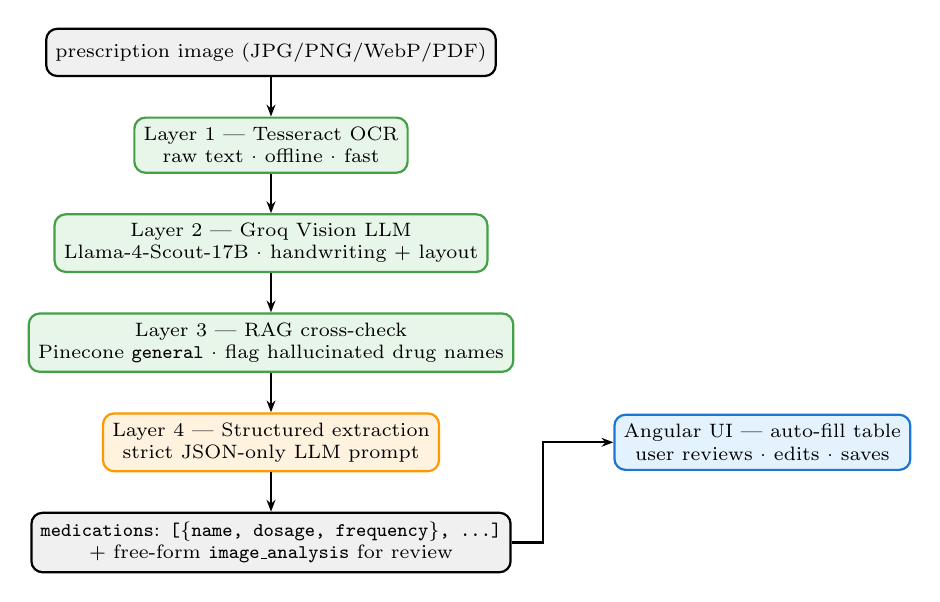
\begin{tikzpicture}[node distance=0.5cm and 0.7cm]
    \node[io] (img) {prescription image (JPG/PNG/WebP/PDF)};
    \node[stage, below=of img] (l1) {Layer 1 --- Tesseract OCR\\\scriptsize raw text · offline · fast};
    \node[stage, below=of l1] (l2) {Layer 2 --- Groq Vision LLM\\\scriptsize Llama-4-Scout-17B · handwriting + layout};
    \node[stage, below=of l2] (l3) {Layer 3 --- RAG cross-check\\\scriptsize Pinecone \texttt{general} · flag hallucinated drug names};
    \node[stage, below=of l3, fill=extfill, draw=extstr] (l4) {Layer 4 --- Structured extraction\\\scriptsize strict JSON-only LLM prompt};
    \node[io, below=of l4] (out) {\texttt{medications}: \texttt{[\{name, dosage, frequency\}, ...]}\\\scriptsize +~free-form \texttt{image\_analysis} for review};
    \draw[flow] (img) -- (l1);
    \draw[flow] (l1) -- (l2);
    \draw[flow] (l2) -- (l3);
    \draw[flow] (l3) -- (l4);
    \draw[flow] (l4) -- (out);
    \node[stage, right=2.2cm of l4, draw=javastr, fill=javafill] (ui) {Angular UI --- auto-fill table\\\scriptsize user reviews · edits · saves};
    \draw[flow] (out.east) -- ++(0.4cm, 0) |- (ui.west);
  \end{tikzpicture}}%
  \vspace{4pt}\\
  \small Three image-analysis layers plus a structured-output call $\rightarrow$ the medications table populates itself.
\end{frame}

% ============================================================================
%  SPEAKER 3 — RITABRATA — RAG Chatbot
% ============================================================================
\section{Ritabrata --- Medical Chatbot}

\begin{frame}{Introduction --- the Medical Chatbot}
  \begin{itemize}
    \item \textbf{Tagline:} An AI health assistant for triage, nutrition, and home care.
    \item \textbf{The problem.} When someone feels unwell, they rarely know how serious it is, what to eat to recover, or when to actually see a doctor. Most consult Google or social media --- noisy, generic, sometimes dangerous advice.
    \item \textbf{The solution.} A conversational assistant that understands symptoms in \emph{text}, \emph{voice}, or a \emph{photo of a medical report} and gives a structured, grounded reply: likely condition, severity level, daily nutrition targets, and a home-management plan. For emergencies it auto-opens a hospital finder and a Call-108 button.
    \item \textbf{Why it matters.} It turns a vague symptom into a useful first step --- bridging \emph{``I don't feel right''} and \emph{``I'm walking into a clinic''}.
  \end{itemize}
  \vfill
  {\scriptsize \textit{Tech stack:} Python · Flask · LangChain · Groq llama-3.3-70b · Pinecone RAG · HuggingFace embeddings · Whisper voice · Tesseract OCR · SQLite}
\end{frame}

\begin{frame}{Main features (1/2)}
  \footnotesize
  \begin{enumerate}
    \item \textbf{Multi-modal input} --- talk to it any way you can describe a symptom.\\
          {\scriptsize text · voice (Whisper) · medical-report photo (OCR)}
    \item \textbf{5-step RAG pipeline} --- symptoms are structured first, then matched against a medical KB before the LLM speaks.\\
          {\scriptsize extract $\rightarrow$ disease ID $\rightarrow$ fallback $\rightarrow$ nutrition $\rightarrow$ severity $\rightarrow$ care}
    \item \textbf{Three-layer severity triage} --- rules (fever, age, duration) + critical keywords + LLM triage, ``worst-of'' so we never under-call an emergency.\\
          {\scriptsize \textcolor{critred}{CRITICAL} · URGENT · MODERATE · MILD}
    \item \textbf{Emergency response} --- CRITICAL auto-opens a red modal with live GPS hospital finder + Call-108 button. Home-care skipped.\\
          {\scriptsize geolocation API · severity-driven UI}
    \item \textbf{Personalised nutrition} --- disease-specific daily macro targets (carbs / protein / fat / fiber / water) stored per user.\\
          {\scriptsize RAG over nutrition.pdf · stored in SQLite}
  \end{enumerate}
\end{frame}

\begin{frame}{Main features (2/2)}
  \footnotesize
  \begin{enumerate}\setcounter{enumi}{5}
    \item \textbf{Cultural meal plans} --- optional cultural-advice route turns the macro targets into a regional 3-meal plan respecting disease restrictions.\\
          {\scriptsize friend's HuggingFace advisor integration}
    \item \textbf{Home-management plan} --- a 7-row table for every MILD / MODERATE / URGENT case: rest, hydration, activity, monitoring, OTC, warning signs.\\
          {\scriptsize LLM-generated, tailored to identified disease}
    \item \textbf{3-layer medical-image OCR} --- Tesseract for fast text, Groq vision (llama-4-scout) for layout, RAG cross-check for medical terms --- fed back into the pipeline.\\
          {\scriptsize handles printed reports, hand-written notes, lab pages}
    \item \textbf{Proactive check-ins} --- 12 hours after a session, the bot asks how you're feeling and re-runs severity --- escalates if worse.\\
          {\scriptsize GET \texttt{/checkin} · POST \texttt{/checkin/reply}}
    \item \textbf{Persistent session memory} --- every session keeps last\_disease, last\_severity, messages, profile, nutrition targets --- bot stays continuous across visits.\\
          {\scriptsize SQLite --- 4 tables, auto-migrating}
  \end{enumerate}
\end{frame}

\begin{frame}{Working diagram --- request lifecycle inside \texttt{run\_pipeline()}}
  \centering
  \adjustbox{max size={\linewidth}{0.72\textheight}}{%
  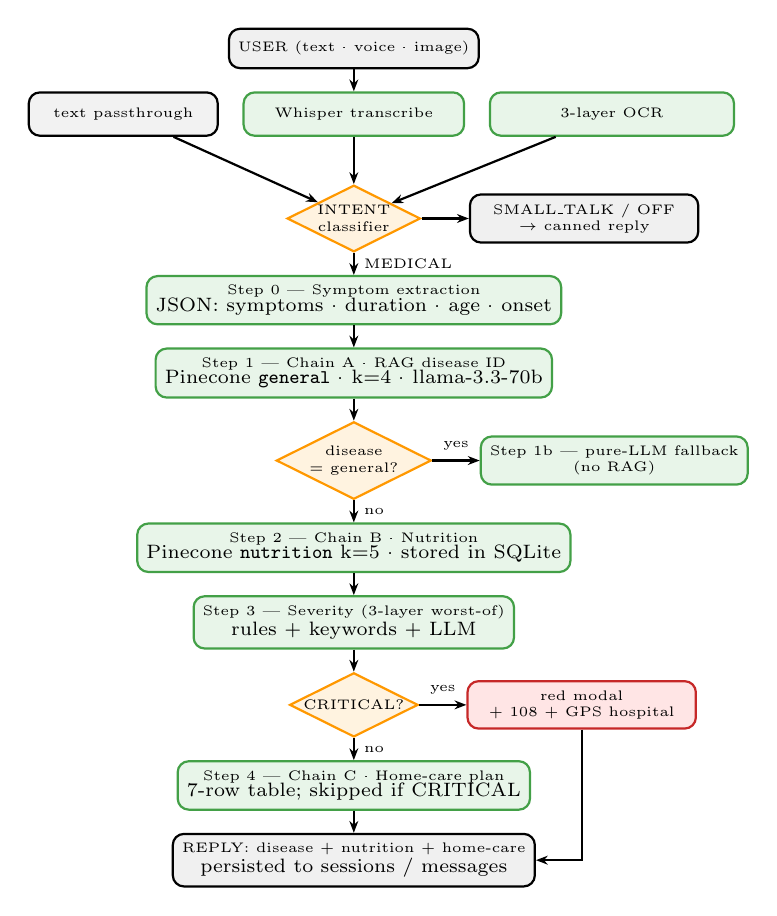
\begin{tikzpicture}[node distance=0.28cm and 0.45cm,
    stage/.append style={minimum width=2.9cm, minimum height=0.55cm, font=\tiny},
    io/.append style={minimum width=2.3cm, minimum height=0.5cm, font=\tiny},
    gate/.append style={inner sep=0.5pt}]
    \node[io] (in) {USER (text · voice · image)};
    \node[stage, below=of in, minimum width=2.8cm, font=\tiny] (whi) {Whisper transcribe};
    \node[stage, right=0.3cm of whi, minimum width=3.1cm, font=\tiny] (ocr) {3-layer OCR};
    \node[stage, left=0.3cm of whi, minimum width=2.4cm, font=\tiny, fill=gray!10, draw=black] (txt) {text passthrough};

    \node[gate, below=0.6cm of whi] (g0) {INTENT\\classifier};
    \node[stage, right=0.6cm of g0, fill=gray!12, draw=black, font=\tiny] (chit) {SMALL\_TALK / OFF\\$\rightarrow$ canned reply};

    \node[stage, below=of g0] (s0) {Step 0 --- Symptom extraction\\\scriptsize JSON: symptoms · duration · age · onset};
    \node[stage, below=of s0] (s1) {Step 1 --- Chain A · RAG disease ID\\\scriptsize Pinecone \texttt{general} · k=4 · llama-3.3-70b};
    \node[gate, below=of s1] (g1) {disease\\= general?};
    \node[stage, right=0.6cm of g1, font=\tiny] (s1b) {Step 1b --- pure-LLM fallback\\(no RAG)};
    \node[stage, below=of g1] (s2) {Step 2 --- Chain B · Nutrition\\\scriptsize Pinecone \texttt{nutrition} k=5 · stored in SQLite};
    \node[stage, below=of s2] (s3) {Step 3 --- Severity (3-layer worst-of)\\\scriptsize rules + keywords + LLM};
    \node[gate, below=of s3] (g2) {CRITICAL?};
    \node[stage, right=0.6cm of g2, fill=red!10, draw=critred, font=\tiny] (modal) {red modal\\+ 108 + GPS hospital};
    \node[stage, below=of g2] (s4) {Step 4 --- Chain C · Home-care plan\\\scriptsize 7-row table; skipped if CRITICAL};
    \node[io, below=of s4] (out) {REPLY: disease + nutrition + home-care\\\scriptsize persisted to sessions / messages};

    \draw[flow] (in) -- (whi);
    \draw[flow] (txt) -- (g0);
    \draw[flow] (whi) -- (g0);
    \draw[flow] (ocr) -- (g0);
    \draw[flow] (g0) -- node[right, font=\tiny]{MEDICAL} (s0);
    \draw[flow] (g0) -- (chit);
    \draw[flow] (s0) -- (s1);
    \draw[flow] (s1) -- (g1);
    \draw[flow] (g1) -- node[above, font=\tiny]{yes} (s1b);
    \draw[flow] (g1) -- node[right, font=\tiny]{no} (s2);
    \draw[flow] (s2) -- (s3);
    \draw[flow] (s3) -- (g2);
    \draw[flow] (g2) -- node[above, font=\tiny]{yes} (modal);
    \draw[flow] (g2) -- node[right, font=\tiny]{no} (s4);
    \draw[flow] (s4) -- (out);
    \draw[flow] (modal.south) |- ($(out.east)+(0.4cm,0)$) -- (out.east);
  \end{tikzpicture}}\\[2pt]
  {\tiny External services: Groq Cloud · Pinecone · HuggingFace embeddings · optional HF advisor.~~~Persistence: SQLite (4 tables)}
\end{frame}

% ============================================================================
%  SPEAKER 4 — ADITI — Cultural Adaptation
% ============================================================================
\section{Aditi --- Cultural Adaptation}

\begin{frame}{Why cultural adaptation is non-optional in India}
  \begin{itemize}
    \item Generic Western diet advice (toast, oatmeal, eggs) doesn't fit an Indian patient who eats rice three meals a day
    \item \textbf{Same symptoms, three patients, three different correct answers:}
    \begin{itemize}\small
      \item Tamil Nadu / Vegetarian $\rightarrow$ idli, sambar, kootu
      \item West Bengal / Non-vegetarian $\rightarrow$ bhaat, machher jhol
      \item Punjab / Vegan $\rightarrow$ makki roti, sarson saag (no ghee/cream)
    \end{itemize}
    \item Wrong advice = user dismisses the entire app
  \end{itemize}
  \vfill
  \begin{exampleblock}{Our position}
    Cultural personalisation is implemented as a \textbf{data contract} that threads from the registration form all the way to the LLM's prompt --- not as a one-off ``if state==X'' switch.
  \end{exampleblock}
\end{frame}

\begin{frame}{Main features --- end-to-end contract}
  \footnotesize
  \begin{enumerate}
    \item \textbf{4 cultural fields collected at registration}\\
          {\scriptsize \texttt{dateOfBirth} (drives age) · \texttt{gender} · \texttt{state} (28 + 8 UTs) · \texttt{dietPreference} (Veg / Non-veg / Vegan / Eggetarian / Jain)}
    \item \textbf{Stored in \texttt{user\_profiles}} on user-service's Postgres --- canonical source of truth
    \item \textbf{Read by chatbot per query} via \texttt{GET /api/v1/users/me} --- always current; profile edits update advice immediately, no re-login
    \item \textbf{Prompt enrichment} with regional examples baked in\\
          {\scriptsize TN $\rightarrow$ idli/sambar/kootu · WB $\rightarrow$ bhaat/posto/shukto · Punjab $\rightarrow$ makki ki roti/sarson}
    \item \textbf{Strict diet rules in prompt + post-check}\\
          {\scriptsize Veg: no meat/fish/eggs. Vegan: no dairy/ghee/butter/cream/honey. Jain: no root vegetables.}
    \item \textbf{Cached meal plans} per (user, session) in \texttt{meal\_plans} SQLite table --- no re-LLM on revisit
    \item \textbf{Optional HuggingFace advisor route} --- teammate's FastAPI service fine-tuned on Indian food data
  \end{enumerate}
\end{frame}

\begin{frame}{Working diagram --- where the cultural context flows}
  \centering
  \adjustbox{max size={\linewidth}{0.78\textheight}}{%
  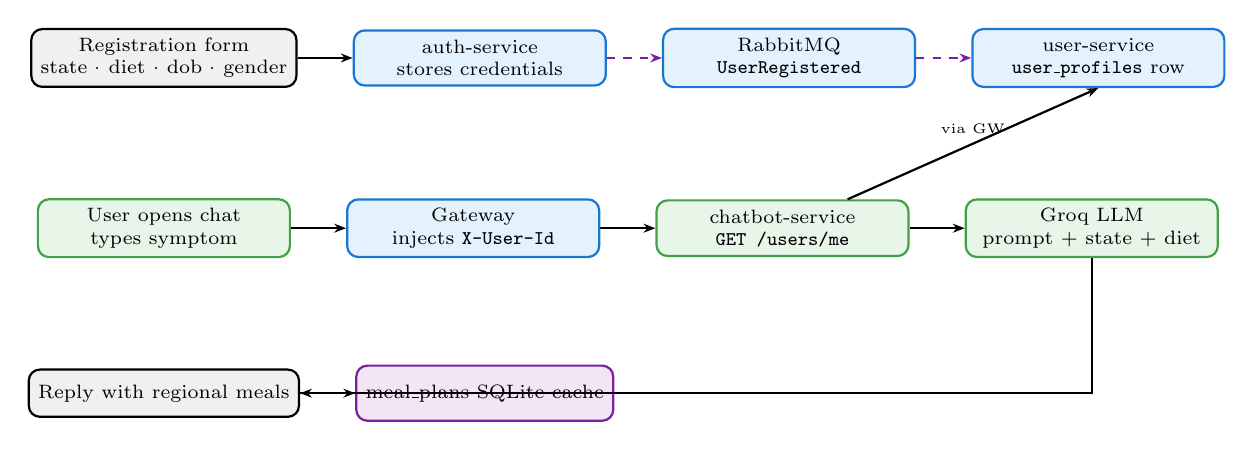
\begin{tikzpicture}[node distance=0.45cm and 0.7cm]
    \node[io] (form) {Registration form\\\scriptsize state · diet · dob · gender};
    \node[stage, right=of form, draw=javastr, fill=javafill] (auth) {auth-service\\\scriptsize stores credentials};
    \node[stage, right=of auth, draw=javastr, fill=javafill] (rmq) {RabbitMQ\\\scriptsize \texttt{UserRegistered}};
    \node[stage, right=of rmq, draw=javastr, fill=javafill] (user) {user-service\\\scriptsize \texttt{user\_profiles} row};
    \node[stage, below=1.4cm of form] (chat) {User opens chat\\\scriptsize types symptom};
    \node[stage, right=of chat, draw=javastr, fill=javafill] (gw) {Gateway\\\scriptsize injects \texttt{X-User-Id}};
    \node[stage, right=of gw] (cb) {chatbot-service\\\scriptsize \texttt{GET /users/me}};
    \node[stage, right=of cb] (llm) {Groq LLM\\\scriptsize prompt + state + diet};
    \node[io, below=1.4cm of chat] (reply) {Reply with regional meals};
    \node[stage, right=of reply, fill=infrafill, draw=infrastr] (cache) {meal\_plans SQLite cache};

    \draw[flow] (form) -- (auth);
    \draw[evt] (auth) -- (rmq);
    \draw[evt] (rmq) -- (user);
    \draw[flow] (chat) -- (gw);
    \draw[flow] (gw) -- (cb);
    \draw[flow] (cb) -- node[above, font=\tiny]{via GW} (user.south);
    \draw[flow] (cb) -- (llm);
    \draw[flow] (llm.south) |- (reply.east);
    \draw[flow] (reply) -- (cache);
  \end{tikzpicture}}\\[6pt]
  {\scriptsize Solid arrows = synchronous HTTP. Dashed = RabbitMQ event. The user-service is the only canonical source of cultural fields; the chatbot reads via the gateway-injected user-ID.}
\end{frame}

% ============================================================================
%  SPEAKER 5 — DEBOSMITA — Backend, APIs, Microservices
% ============================================================================
\section{Debosmita --- Backend \& APIs}

\begin{frame}{Eight services --- ports + responsibilities}
  \footnotesize
  \begin{center}
  \begin{tabular}{>{\bfseries}l l l}
    \toprule
    Service & Port & Responsibility \\
    \midrule
    Eureka & 8761 & Service registry (every service heartbeats here) \\
    API Gateway & 8080 & Single entry point; validates JWTs; injects \texttt{X-User-Id} \\
    Auth Service & 8081 & Login, OTP, refresh tokens, blacklist \\
    User Service & 8082 & Profile, family hub, emergency contacts \\
    Health Service & 8083 & Vitals, mood, FHIR export, health-score \\
    Prescription Service & 8084 & Prescriptions, medications, drug interactions, appointments \\
    Notification Service & 8085 & Reminders, alerts, in-app notifications \\
    Chatbot Service & 8086 & Python Flask · RAG · OCR · severity \\
    \bottomrule
  \end{tabular}
  \end{center}
  \vspace{4pt}
  \begin{block}{Communication topology --- two channels, only two}
    \small \textbf{Sync:} clients hit Gateway $\rightarrow$ Eureka load-balances to service. \quad \textbf{No direct service-to-service HTTP.}\\
    \textbf{Async:} RabbitMQ topic exchange \texttt{medihelp.events} --- six event types.
  \end{block}
\end{frame}

\begin{frame}{Event listeners --- the six RabbitMQ event types}
  \footnotesize
  \begin{tabular}{ll p{6.5cm}}
    \toprule
    \textbf{Event} & \textbf{Producer} & \textbf{Consumer + behaviour} \\
    \midrule
    \texttt{UserRegistered}   & auth & user-service creates default profile \\
    \texttt{MedicationReminder} & prescription (scheduler) & notification-service queues + delivers \\
    \texttt{AppointmentReminder} & prescription (scheduler) & notification-service queues + delivers \\
    \texttt{EmergencySos}     & health  & user-service notifies family-hub members \\
    \texttt{VitalsAnomaly}    & health  & notification-service raises alert (BP > 180 etc.) \\
    \texttt{Notification}     & any     & notification-service generic catch-all \\
    \bottomrule
  \end{tabular}
  \vfill
  \begin{exampleblock}{Why events, not synchronous calls?}
    \small If notification-service is down, the RabbitMQ queue holds the messages. When it comes back, it consumes them. \textbf{Resilience for free.}\\
    No distributed transactions --- we accept \emph{eventual consistency}.
  \end{exampleblock}
\end{frame}

\begin{frame}[fragile]{JWT --- validated only at the Gateway}
  Downstream services \textbf{never parse JWTs}. The gateway:
  \begin{enumerate}\small
    \item Validates token signature
    \item Checks Redis blacklist (added on logout via \texttt{jti})
    \item \textbf{Strips} the Authorization header, injects three trusted headers
  \end{enumerate}
  \vspace{2pt}
  \begin{lstlisting}[basicstyle=\ttfamily\scriptsize, frame=single, framerule=0.4pt]
@GetMapping("/me")
public ApiResponse<UserProfile> getMe(
    @RequestHeader("X-User-Id") String userId) {
  return ApiResponse.success(userService.getProfile(userId));
}
  \end{lstlisting}
  \vfill
  \begin{itemize}\small
    \item Polyglot benefit: Python chatbot reads the same header --- no JWT library duplication
    \item \texttt{PUBLIC\_PATHS} allow-list (register, login, refresh, public/**) skips auth
  \end{itemize}
\end{frame}

\begin{frame}{Refresh-token rotation --- 15-min access + 60-day refresh}
  \begin{columns}[T]
    \column{0.5\textwidth}
    \footnotesize
    \textbf{Flow on \texttt{POST /auth/refresh}:}
    \begin{enumerate}
      \item Look up refresh-token hash in DB
      \item Verify not revoked, not expired
      \item \alert{Mark old row \texttt{revoked = true}}
      \item Generate \emph{new} pair; store hash of new refresh in new row
      \item Return both
    \end{enumerate}
    \vspace{4pt}
    \textbf{Why rotate?} A stolen token works \emph{once} --- second use fails because row is revoked, and the legitimate user is forced to re-login (signal that something is wrong).
    \column{0.5\textwidth}
    \footnotesize
    \textbf{Angular HttpInterceptor deduplication:}
    \begin{itemize}
      \item Multiple in-flight requests can hit 401 simultaneously
      \item Without dedup, each fires its own refresh $\rightarrow$ race
      \item \texttt{refreshTokenShared} \texttt{BehaviorSubject} = first 401 starts refresh; others subscribe and retry on completion
      \item Falls through to \texttt{/login} only if refresh itself fails
    \end{itemize}
  \end{columns}
\end{frame}

\begin{frame}{Health charts + the Fitbit story}
  \begin{columns}[T]
    \column{0.5\textwidth}
    \footnotesize
    \textbf{Vital trends (working):}
    \begin{itemize}
      \item \texttt{GET /api/v1/health/vitals/trends?type=...\&days=7}
      \item Returns aggregate: average, min, max, readingsCount, periodDays
      \item Frontend renders via \texttt{@swimlane/ngx-charts} v22 (pinned for Angular 17)
      \item Heart rate · BP (dual line) · Weight · Temperature
    \end{itemize}
    \column{0.5\textwidth}
    \footnotesize
    \textbf{Why Fitbit integration was descoped:}
    \begin{itemize}
      \item Fitbit OAuth callback URL \emph{requires HTTPS} on a registered domain
      \item Our free Azure VM has only an IP, HTTP only --- Fitbit dev portal refuses to accept it
      \item Data ingestion needs a batched endpoint (\texttt{POST /vitals/batch}) --- not built yet
      \item Rate-limited at 150 req/h per user $\rightarrow$ needs a per-user scheduled sync job
      \item OAuth token storage adds compliance scope (HIPAA-adjacent)
    \end{itemize}
    \vspace{2pt}
    \alert{Verdict:} \emph{deployment-infrastructure problem}, not application code. Spec'd in our thesis future-work chapter.
  \end{columns}
\end{frame}

% ============================================================================
%  SPEAKER 6 — SOUVIK — Database Architecture
% ============================================================================
\section{Souvik --- Database Architecture}

\begin{frame}{Service-to-database mapping}
  \centering
  \footnotesize
  \begin{tabular}{>{\bfseries}l c p{6.3cm}}
    \toprule
    Service & Database & Purpose \\
    \midrule
    Auth Service & SQL & User login, signup, authentication \\
    Prescription Service & SQL & Store prescriptions and OCR medicine data \\
    Medication Tracker & SQL & Medicine reminders and adherence tracking \\
    Nutrition Service & SQL & Diet and nutrition recommendations \\
    Journal Service & SQL & Encrypted personal health journals \\
    Health Service & MongoDB & Dynamic health records and symptom data \\
    AI Chatbot Service & SQLite & Chatbot conversation history \\
    \bottomrule
  \end{tabular}
  \vfill
  \begin{exampleblock}{Design rule}
    \small One database per service --- enforced service boundaries, independent schema evolution, failure isolation. \emph{Cost:} no foreign keys across service boundaries. \emph{Workaround:} eventual consistency via RabbitMQ events.
  \end{exampleblock}
\end{frame}

\begin{frame}{Database schema (1/3)}
  \centering
  \includegraphics[width=0.95\linewidth, height=0.82\textheight, keepaspectratio]{Images/souvik-slide-2.png}
\end{frame}

\begin{frame}{Database schema (2/3)}
  \centering
  \includegraphics[width=0.95\linewidth, height=0.82\textheight, keepaspectratio]{Images/souvik-slide-3.png}
\end{frame}

\begin{frame}{Database schema (3/3)}
  \centering
  \includegraphics[width=0.95\linewidth, height=0.82\textheight, keepaspectratio]{Images/souvik-slide-4.png}
\end{frame}

\begin{frame}{Advantages of our database design}
  \begin{enumerate}
    \item \textbf{Microservice-based architecture}
    \begin{itemize}\small
      \item Each service works independently
      \item Easier to maintain and update
      \item Better modularity
    \end{itemize}
    \item \textbf{Optimised database selection}
    \begin{itemize}\small
      \item SQL for structured healthcare data
      \item MongoDB for flexible health records
      \item SQLite for lightweight chatbot storage
    \end{itemize}
    \item \textbf{Scalability}
    \begin{itemize}\small
      \item Services can scale independently
      \item Handles increasing users efficiently
    \end{itemize}
  \end{enumerate}
\end{frame}

% ============================================================================
%  SPEAKER 7 — SUBHRAJIT — Integration & Deployment
% ============================================================================
\section{Subhrajit --- Integration \& Deployment}

\begin{frame}{How it wires together --- system topology}
  \centering
  \adjustbox{max size={\linewidth}{0.72\textheight}}{%
  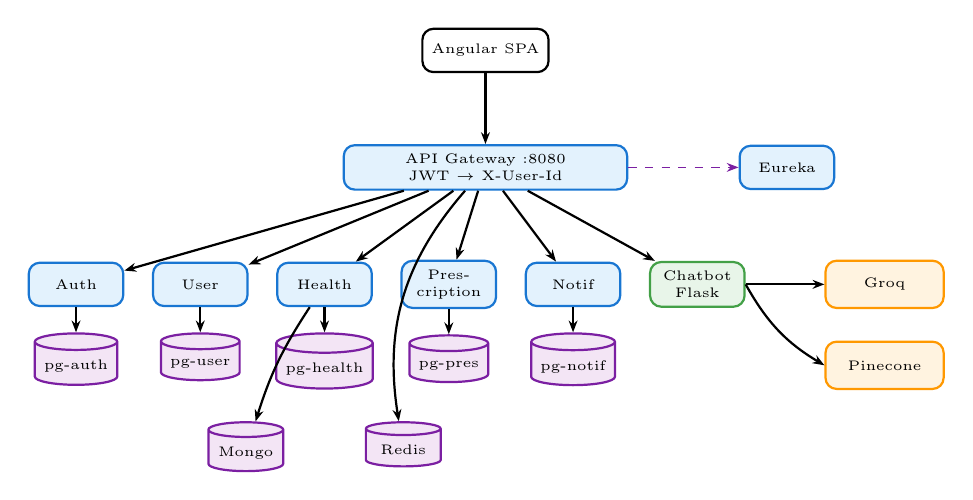
\begin{tikzpicture}[node distance=0.32cm and 0.35cm,
    jbox/.append style={minimum width=1.2cm, minimum height=0.55cm, font=\tiny},
    pybox/.append style={minimum width=1.2cm, minimum height=0.55cm, font=\tiny},
    infrabox/.append style={minimum width=0.95cm, minimum height=0.55cm, font=\tiny}]
    \node[jbox, fill=white, draw=black] (br) {Angular SPA};
    \node[jbox, below=0.9cm of br, minimum width=3.6cm] (gw) {API Gateway~:8080\\\tiny JWT $\rightarrow$ X-User-Id};
    \node[jbox, right=1.4cm of gw] (eu) {Eureka};
    \node[jbox, below=0.9cm of gw, xshift=-5.2cm] (auth) {Auth};
    \node[jbox, right=of auth] (user) {User};
    \node[jbox, right=of user] (health) {Health};
    \node[jbox, right=of health] (pres) {Pres-\\cription};
    \node[jbox, right=of pres] (notif) {Notif};
    \node[pybox, right=of notif] (chat) {Chatbot\\\tiny Flask};
    \node[infrabox, below=of auth] (pga) {pg-auth};
    \node[infrabox, below=of user] (pgu) {pg-user};
    \node[infrabox, below=of health] (pgh) {pg-health};
    \node[infrabox, below=of pres] (pgp) {pg-pres};
    \node[infrabox, below=of notif] (pgn) {pg-notif};
    \node[infrabox, below=0.4cm of pgh, xshift=-1cm] (mongo) {Mongo};
    \node[infrabox, below=0.4cm of pgh, xshift=1cm] (redis) {Redis};
    \node[extbox, right=1.0cm of chat] (groq) {Groq};
    \node[extbox, below=0.4cm of groq] (pine) {Pinecone};
    \draw[flow] (br) -- (gw);
    \draw[flow] (gw) -- (auth);
    \draw[flow] (gw) -- (user);
    \draw[flow] (gw) -- (health);
    \draw[flow] (gw) -- (pres);
    \draw[flow] (gw) -- (notif);
    \draw[flow] (gw) -- (chat);
    \draw[evt, thin] (gw) -- (eu);
    \draw[flow] (auth) -- (pga);
    \draw[flow] (user) -- (pgu);
    \draw[flow] (health) -- (pgh);
    \draw[flow] (pres) -- (pgp);
    \draw[flow] (notif) -- (pgn);
    \draw[flow] (health) to[bend right=8] (mongo);
    \draw[flow] (gw) to[bend right=25] (redis);
    \draw[flow] (chat) -- (groq);
    \draw[flow] (chat.east) to[bend right=15] (pine.west);
  \end{tikzpicture}}
  \vfill
  {\scriptsize Eureka registers every service. Gateway resolves \texttt{lb://service-name} via Eureka and load-balances. Dashed lines = Eureka heartbeats (RabbitMQ events omitted for clarity).}
\end{frame}

\begin{frame}{Deployment on a single Azure VM}
  \begin{columns}[T]
    \column{0.55\textwidth}
    \footnotesize
    \textbf{What's on the VM (98.70.34.96):}
    \begin{itemize}
      \item Ubuntu 24.04 · B2s · 2 vCPU · 4 GB RAM
      \item Docker for stateful infra (5 Postgres + Mongo + Redis + RabbitMQ)
      \item 6 Java fat JARs + 1 Python Flask + Eureka
      \item nginx serving the Angular dist on port 80
      \item nginx reverse-proxies \texttt{/api/*} to gateway $\rightarrow$ same-origin, no CORS drama
    \end{itemize}
    \column{0.45\textwidth}
    \footnotesize
    \textbf{systemd auto-restart} (single unit):
    \begin{itemize}
      \item \texttt{ExecStart=/bin/bash start-all.sh}
      \item \texttt{Type=forking · RemainAfterExit=yes}
      \item \texttt{Restart=on-failure · RestartSec=30}
    \end{itemize}
    \vspace{4pt}
    \textbf{Redeploy} = git pull + \texttt{systemctl restart medihelp} + smoke test. \textasciitilde90s.
  \end{columns}
\end{frame}

\begin{frame}{Observability + smoke test}
  \begin{columns}[T]
    \column{0.5\textwidth}
    \footnotesize
    \textbf{Self-hosted Prometheus + Grafana} (Docker compose):
    \begin{itemize}
      \item Prometheus scrapes \texttt{/actuator/prometheus} every 15s
      \item Grafana dashboard auto-provisioned from JSON
      \item Panels: heap, RPS, p95 latency, GC pauses, threads, services-up
    \end{itemize}
    \vspace{4pt}
    \textbf{Observed values on VM:}
    \begin{itemize}
      \item p95 latency \textless 100 ms (non-LLM endpoints)
      \item Chatbot \texttt{/get}: 8--12 s (5 sequential LLM calls)
      \item Heap well under \texttt{-Xmx256m}
    \end{itemize}
    \column{0.5\textwidth}
    \footnotesize
    \textbf{Smoke test} (\texttt{deploy/scripts/smoke-test.sh}):
    \begin{itemize}
      \item register $\rightarrow$ OTP grep $\rightarrow$ verify $\rightarrow$ login
      \item POST vital · POST mood · chatbot \texttt{/get}
      \item All 8 checks must pass for production readiness
    \end{itemize}
    \vspace{4pt}
    \begin{block}{}\centering
\includegraphics[width=\linewidth]{Images/17-grafana.png}\end{block}
  \end{columns}
\end{frame}

\begin{frame}{Conclusion + future work}
  \textbf{What we built:}
  \begin{itemize}\small
    \item 8 microservices · \textasciitilde18\,000 LoC · deployed on a single VM
    \item RAG chatbot with off-topic gate, cultural advice, drug-interaction safety
    \item HL7 FHIR R4 export · mood journal · family hub · emergency SOS with geolocation
    \item Self-hosted Prometheus + Grafana observability
  \end{itemize}
  \textbf{Honest limitations:} single-VM SPOF · English-only output · OTP delivery restricted to verified address · no formal medical review · HTTP only (Fitbit OAuth blocker).\\[6pt]
  \textbf{Future work:}
  \begin{itemize}\small
    \item TLS deployment $\rightarrow$ Fitbit / Apple Health / Google Fit integration
    \item Multi-LLM fallback (Anthropic Claude, OpenAI) for Groq rate-limit days
    \item Conversational memory across sessions; streaming responses
    \item Kubernetes + multi-region for higher availability
    \item HIPAA / GDPR formal compliance audit
  \end{itemize}
  \vfill
  \centering \alert{\textbf{Thank you. Questions?}}
\end{frame}

\end{document}
